
\chapter{Design and Implementation of Air pollution Monitoring System}

  %understanding air pollution used complex and stationary equipment which collects data and used these data for analyzing, but things have changed after the low cost, easy to use, portable sensors came in markets \cite{Snyder2013}.
  
The use of complex, expensive, and stationary monitors for collecting and analyzing pollutant data began soon after the 1970 Clean Air Act came into action in the USA \cite{Daly2007}. Ever since then researchers and environmentalists have been interested in studying the pollution data and its effects. This became even more popular after the development of low cost, easy to use, portable sensors in the market \cite{Snyder2013}. In our research work, we have attempted to fill the gap for understanding the quality of the data obtained from low-cost sensors by comparing these with the official monitoring system in the city of Prince George. 

In this chapter, we share our hands-on experience in the design, development, integration, and operation of the air pollution monitoring system using low-cost sensors from the market. We have also build a visualization tool for effective data representation which is explained at the end of the chapter.



\section{Design Goals}

For the development of a reliable and simple pollution monitoring system, these are the steps we followed to make the system efficient. These goals are very unique to our work and are listed as follows: 

%The first step towards creating the system was to identify and recognize the components which could be used to make the system. There are many factors which need to be considered for the development of a simple yet reliable system. In this section, I will share the idea that we wanted to achieve in building our air pollution system. 

\begin {enumerate}
%\item{Pollution monitoring for EPA criteria pollutant}

\item{Sensor Selection}

There are different kinds of sensors available in the market for measuring each pollutant. Selecting the right kind for obtaining accurate data was one of the challenging tasks. We referred to the Air Sensor Guidebook by US Environmental Protection Agency (EPA)\cite{airsensorguidebook} that came with guidelines that we followed before purchasing the sensor. One of the main factors that we looked at in the sensor is for accuracy. Keeping this in mind, we researched different available sensors in the market and selected the ones which we felt would meet our needs. 

%The very first task is to figure out which all sensors need to be included for understanding the air quality. There are sensors available in the market for the measurement of almost all types of gases in the atmosphere. It should be very clear that which all gases need to be measured and this depends from region to region as in certain places the concentration of a particular gas is more. 

\item{Processor Platform Selection}

To make the system work there needs to be a processor and platform. Choosing which processor to work with was the next task which we dealt with by answering the questions like:
\begin{itemize}
   \item Whether we wanted our system to be simple or complex? 
  \item Whether it is open-source in hardware and software? 
  \item The ease of programming
  \item How easily can the processor be available? 
  \item What is the cost?.

\end{itemize}

By answering each of these gave us clear criteria for selecting the platform.


\item{Communication Module}

Once the sensors and platform were identified the next step was to find out a way how the data collected from the processor should be transferred to a database. We wanted the system to be wireless and for that, either Bluetooth or Wi-Fi module can be used. We wanted instantaneous data representation and the Wi-Fi module was a better choice for that purpose. 

%As the system is completely based on wireless sensors, the data transmission is another crucial factor. The communication between the server and the sensors should be taken into consideration. The collected data from the sensors should be transferred to a sever. For that, communication module can be either Wi-Fi or bluetooth module.
 
%\item {Reliability}

%The success of the system depends upon how reliable the system is. The value which we obtain from the sensor should make sense to the audience. There will be a lot of noise coming with the  collection of data, the sensor should have the ability to remove the noise data or it should allow the programmer to make changes or apply certain algorithm so that the data sets will be refined.

\item {Easy Integration}

The integration of sensors with the Arduino platform is the next important factor that needs to be addressed. Some sensors can be easily integrated with any processor but others need driver code to be written to work with the processor. Also, the presence of one sensor should not affect the other sensors, which will result in data integrity problems.

\item {Printed Circuit Board}

The initial circuit was built on a wired breadboard to create a prototype of the system. By working on a breadboard made it easy to experiment with different sensors. Once we have identified how each sensor should be placed in a breadboard arrangement the final version should be transformed into a Printed Circuit Board (PCB). By transforming the circuit design into a PCB makes the circuit stable, reliable, and robust.


\item {Maintenance}

The next goal which we wanted to achieve was easy replication of hardware modules in case of any damage. For this we wanted the system to be "plug-and-play" model so that in case of any hardware issue, the debugging will not be challenging. We have also selected the hardware modules based on their availability in the market so that replacement will be quick.

%In case of any damage in sensor it should be easily replaceable which means the complete system should be a plug and play type model. In building up such a model will help in debugging the problems caused by sensors if any. It should also be considered that the sensors selected for the system should be easily available in market so that it can be replaced in case of any damage. The idea behind creating such a system is that it can be replicated by anyone without even knowing the dept knowledge. The system should be designed in such a way that it should use the most available sensors and processors in the market.The programming part of the sensors to processor will be easy if the selection of processor is simple. This could definitely bring down a lot of work done at the hardware level.

\item {Low Cost}

The final factor is cost. The price range for the hardware modules in the market varies from $\$20 $ to $\$800 $ per module in the category of low-cost sensor networks. We wanted to create a low-cost system that is affordable and set a target of under $\$400$ for the entire pollution monitoring system.
%Within the available sensors in the market one could find sensors ranging from a very low price to costliest of all. There was a budget set for the the complete system and finding the right sensors with the affordable cost is one crucial factor.
\end{enumerate}


%\section{Targeted Pollutants}

%Our surrounding is filled with various gases and will become harmful if the concentration increases to an undesired level. We need to carefully identify which pollutant is dominant in a particular area and select the pollutant to be measured accordingly. In this research project, we are measuring the pollutants in the city of Prince George. The main pollutants of interests are  $PM_{2.5}$, $PM_{10}$, $O_3$, $NO_2$, and $CO$. We have also measured the environmental factors like temperature and humidity along with the pollutants. 
% The main idea here is to make the public aware on the dominant pollutant and the extend of health hazard caused by these gases. %This can be identified through different indexes know as Air Quality Health Index  (AQHI) which is a scale from one to ten developed by health and environmental professionals \cite{faq} and Air Quality Index (AQI) which gives the level of air quality status in an area \cite{Asha2017}.

%In this project, we are measuring the pollutants in the city of Prince George and here the main pollutants of interests are  $PM_{2.5}$, $PM_{10}$, $O_3$, $NO_2$, and $CO$. We have also measured the environmental factors like temperature and humidity along with the pollutants.

%On the development of a air pollution system measurement of all the gases in the atmosphere is not necessary as the collected data from all the sensor will make no sense to the public. 
\par 

%The development of such indexes by the scientists will give the general public more idea of the pollution. The main gases to be included for the measurement for the indexes are  $PM_{2.5}$, $O_3$, $NO_2$, and $CO$ along with temperature and humidity sensor for awareness. These gases are mainly caused due to industrialization, urbanization and motorization \cite{Saha1952}. Industrial and vehicles release greenhouse emissions which are largely responsible for air pollution \cite{ internet}. The sensors thus can be limited to five which will also make the system compact.

\section{System Architecture}
    

     In this section, we describe the design process for a low-cost air pollution monitoring system which can be categorized into system hardware architecture and system software architecture. The system is designed in such a way that the processor module collects the data through the sensors and transfers it into a database from where it is visualized. There is also a calibration procedure required which will be explained in the next chapter.
     \begin{figure}[h]
      \begin{center}
      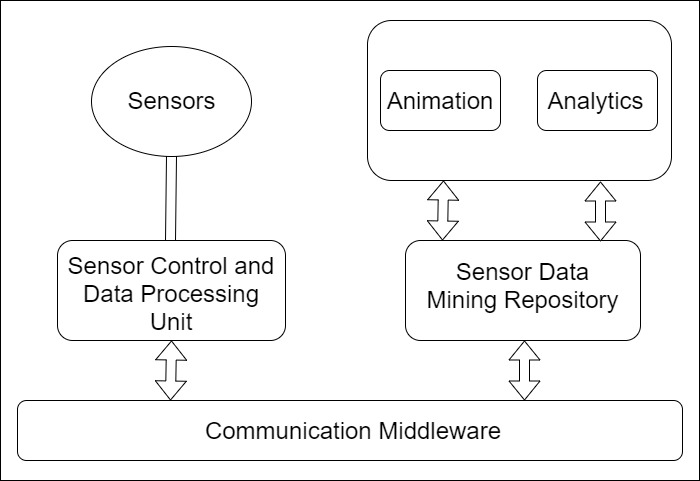
\includegraphics[scale=0.65]{images/figure2.png}
      \end{center}
      
      \caption{System overview}
      \label{overview}
  
    \end{figure}

  \hspace{1 cm}


    The system hardware section includes multiple sensors, the processor, and also the wireless communication module for transmitting and receiving signals. We will also discuss the air pollution visualization tool which mainly focuses on the representation of the data. The overview of the system is as shown in figure \ref{overview} and each part along with the sensor specification, implementation, and design will be discussed further in the section. 
    
    In this research project, we are measuring the pollutants in the city of Prince George. The main pollutants of interests are  $PM_{2.5}$, $PM_{10}$, $O_3$, $NO_2$, and $CO$. We have also measured the environmental variables like temperature and humidity along with the pollutants. 

 \section{Hardware Architecture}
  
\subsection{Sensor Control and Data Processing Unit}

This is the main hardware component for pollution monitoring as it is where all the other sub-modules are connected including the communication middleware. The main function handled by this module are as follows:

\begin{enumerate}

\item Control the sensors in collecting data.
\item Filter and process the collected data 
\item Communicate and forward the data to the server.
\item Provide the necessary power for all the hardware connected to it.

\end{enumerate}
For simplicity and ease of programming, we have selected a popular processor platform, the Arduino Ethernet board which has an ATmega328 microcontroller as shown in Fig.\ref{Arduino}. 

\begin{figure}[h]
  \begin{center}
  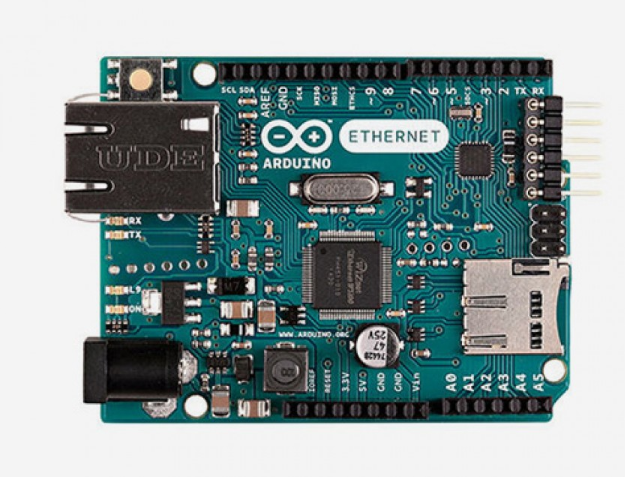
\includegraphics[scale=0.70]{./images/figure3.png}
  \end{center}
  \caption{Arduino Ethernet Board}
  \label{Arduino}
\end{figure}

Arduino is an open-source physical computing platform that is divided into two parts, one is the hardware which is the board itself to which the external components are added and the other is the software which is the development environment for the programming. It is very simple to use the board with many external devices such as sensors or actuators and is widely used by researchers. There are different features which makes Arduino popular and can be listed as \cite{Banzi2008}:


\begin{enumerate}


  \item  Arduino is multi-platform and can be used with Windows, MacOS, and Linux.

  \item The program is uploaded to the module via USB cable.
  \item It has many I/O ports for interfacing external sensor hardware.

  \item It is open-source hardware and software and the code can be easily downloaded.
  
  \item There is an Integrated Development Environment (IDE) which is used as an interface for communicating with the hardware and is very simple.
  
  \item There is an active Arduino forum in which many researchers and developers contribute their ideas and will help in trouble shooting.
  
  \item The cost of the hardware is very low (under 60 CAD) and is easily available.
  
\end{enumerate}


\begin{table}[h]
  
  
  \begin{tabularx}{\columnwidth}{X|X}
      \hline
      Description                 & specification    \\
      \hline
      Microcontroller & ATmega328P \\
      Operating Voltage & 5V\\
      Input Voltage Plug (recommended) & 7-12V\\
      Input Voltage Plug (limits)       & 6-20V\\
      Input Voltage PoE (limits)        & 36-57V \\
      Digital I/O Pins    & 14 (of which 4 provide PWM output)     \\
      Analog Input Pins & 6\\
      Flash Memory & 32 KB (ATmega328P) of which 0.5 KB used by bootloader\\
      SRAM     & 2 KB (ATmega328P)\\
      EEPROM   & 1 KB (ATmega328P) \\
      Clock Speed  & 16 MHz\\
      \hline
    
  \end{tabularx}
  \caption{Technical specification}
  \label{table:Technical specification}
\end{table}
 
The board can be powered either by using a FTDI cable/USB serial connector, external power supply or using a optical Power Over ethernet module (PoE). The detailed specification\cite{Guti2017} of the board is given in the table \ref{table:Technical specification}. These specifications give the freedom for researchers to explore different electronic devices easily. The board is programmed using the Arduino Integrated Development Environment (IDE) which uses an embedded C language.




\subsection{Sensor}

%Sensor networks are instruments useful to detect the conditions in remote places in the physical world in environmental monitoring applications such as pollution monitoring, transportation management, intrusion detection, and many more \cite{Jung2011}. With constant development in the electronics industry, it is possible to collect data remotely and this data can be transferred to a required platform within a short time.

%There are different sensors available in the market which can measure the pollutants and display the value, but the idea here is to select the one which is of low cost and also gives the most accurate values.
In chapter two we have described the various categories of sensor networks and how effectively these can be used in different platforms. In this section, we will be giving an idea of different sensors available in the market and the sensors which we selected for this research project.
There are a variety of options available for sensors to monitor the various pollutants. One such category is the Metal Oxide Semiconductor (MOS) gas sensor also known as the semiconductor gas sensor, which is used to detect the concentration of hazardous gases in the atmosphere. The most popular series available in the market for this category are MQ-XX sensors which are popular for their wide detecting scope, long life, stability, high sensitivity, fast response, and also simple drive circuit \cite{Data2012}. The sensing material is made of either from Aluminium Oxide ($ Al_{2}O_{3}$) or Tungsten Trioxide ($WO_3$) based ceramic and has a coating of Tin Oxide ($ SnO_{2} $) that acts as the sensing material for the desired gas. 

The sensing element is heated by Platinum wires which are connected to leads made of Nickel-Chromium. The gas to be detected has a specific temperature at which it is ionized and the task of the sensor is to work at that temperature. Once the gas is ionized it will be absorbed by the sensing material which changes its resistance and in turn changes the voltage across the sensor and can be read by the microcontroller \cite{gassensor}. The voltage value along with a reference voltage is used to determine the resistance of the sensor. Once the resistance of the sensor is known then by using a calibrated sensitivity curve, the concentration can be found. 

Another popular MOS sensor that we explored was MICS, which is MEMS-based whose mode of operation is similar to the sensor above as both of them are metal oxide. Here, oxidizing gas or the pollutant gas adds to the insulative oxygen species causing the resistance to increase \cite{SGXSensortech}.
 We also considered optical sensors which are spectroscopic devices which use light scattering principles to find the concentration of pollutants. These sensors are known for its capability to detect particulate matter of different sizes and is one of the recent innovations in the field of air quality monitoring. High responsivity, reliability, and long life are the main highlights of this type of sensor.
 
 
 \subsubsection{Selected Sensors}

 After understanding the wide range of sensor options in the market the sensors that were selected are listed below: 
 \begin{enumerate}

  \item MQ-2 Sensor: This is a semiconductor gas sensor which has an electrochemical sensor which detects multiple gases such as Carbon monoxide, LPG, methane, and combustible steam. The sensor is connected in series with a variable resistor to form a voltage divider circuit and the variable resistor is used to change the sensitivity. The range of detection of gases is from 100ppm to 10,000 ppm and has a high sensitivity and fast response time. The sensor is small and portable and provides simple integration with the Arduino platform. %The sensitivity curve for MQ-2 is shown for different types of gases, where $R_{o}$ is the sensor resistance in clean air and $R_{s}$ is the sensor resistance when exposed to gas.
\begin{comment}
\begin{figure}[h]
  \begin{center}
  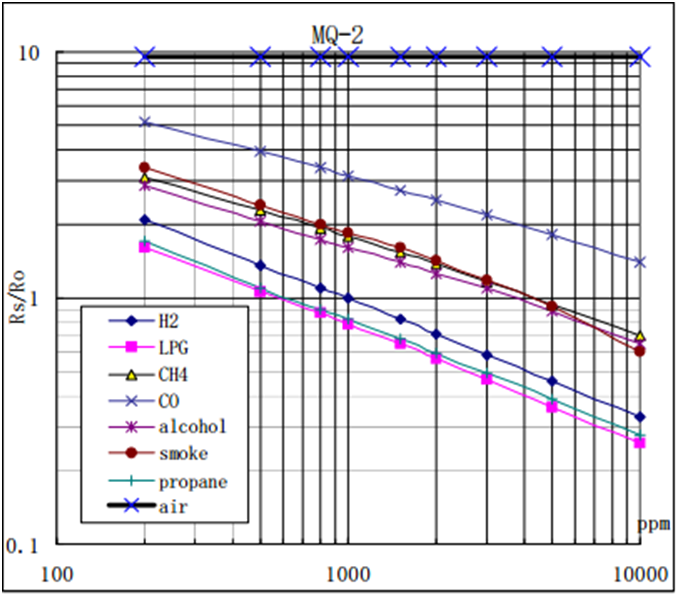
\includegraphics[scale=0.40]{./images/figure1.png}
  \end{center}
 
  \caption{Sensitivity characteristics curve \cite{Data2012}}
  
  \label{curve}

\end{figure}
From the curve in Fig.\ref{curve}, the voltage across the sensor is found out depending on which gas one wants to detect and there after using this voltage value the concentration of pollutant is calculated. The range of detection of gas is from 100ppm to 10,000 ppm and has a high sensitivity and fast response time. The sensor is small and portable and provides integration in famous MCU platforms like arduino, raspberry pi etc. 
\end{comment}
\item MQ-131: Sensor used for ozone detection. The operation of the sensor is similar to MQ-2 sensor. It decreases the resistance when exposed to ozone and becomes more conductive when exposed to large concentration of the gas. This can be used to measure the concentration of ozone in air. The detecting concentration range is from 10ppb to 2 ppm of ozone and also has a fast response time and long life. 

The reference system in downtown uses an API model 400 ozone monitor for the city measurement\cite{Environment2010}. The Figure \ref{Ozonesensor} shows the picture of the Ozone sensor used for measurement at the reference station as well as in our low-cost sensor system.
  
\begin{figure}[h]
  \begin{center}
  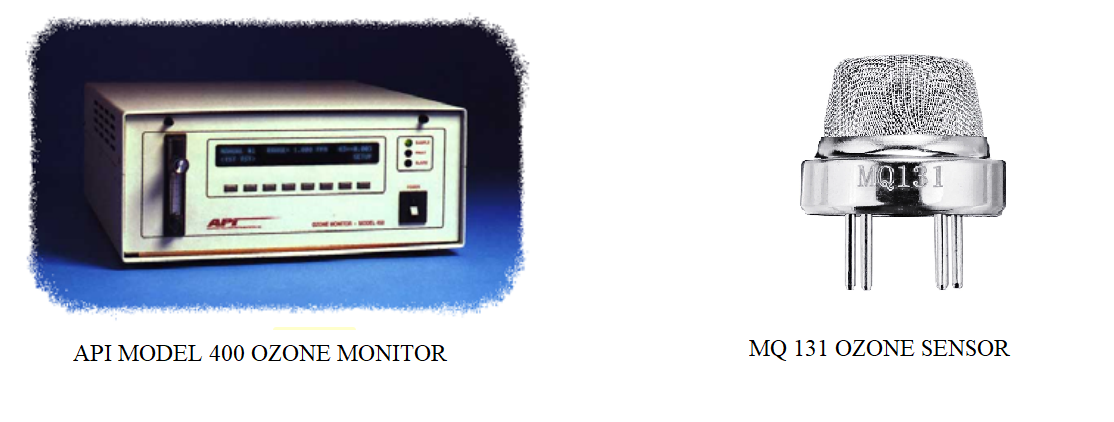
\includegraphics[scale=0.70]{images/figure30.png}
  \end{center}
  \caption{Ozone sensors used for measurement}
  \label{Ozonesensor}
\end{figure}
\hspace{1 cm}

\item MICS-2714: This is a robust MEMS sensor used for the detection of Nitrogen dioxide ($NO_2$). The detection range is from 0.05 to 10 ppm and has a response time of 10 seconds. The sensor is comparatively small and of low cost. The reference system located in Prince George plaza 400 is API $NO_{x}$ monitor \cite{Environment2010} which uses chemiluminesence principle to measure the pollutant . The figure \ref{Nitrogensensor} shows the image of both the sensors for detecting the pollutant.
  
  
  \begin{figure}[h]
   \begin{center}
   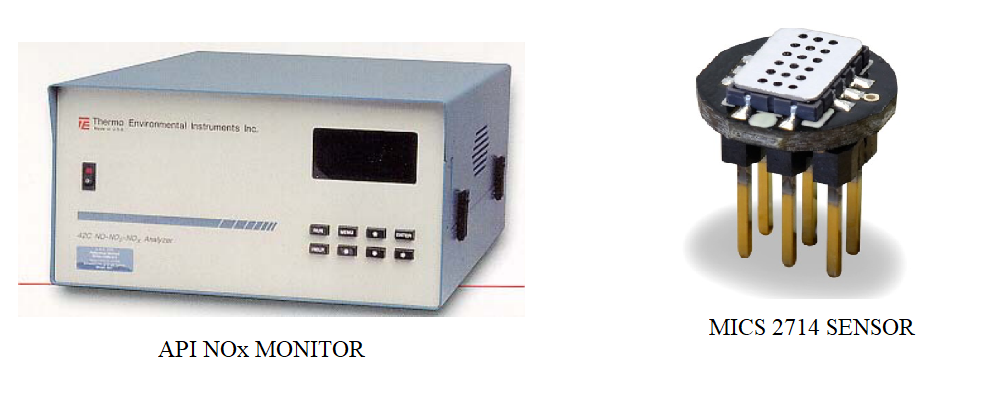
\includegraphics[scale=0.70]{images/figure31.png}
   \end{center}
   \caption{Nitrogen Sensor used for measurement}
 \label{Nitrogensensor}
\end{figure}
  
  

\item  PPD42NS Particulate sensor: The sensor detects particulate matter through the light scattering mechanism and consists of an infrared LED positioned at a forward angle to a photodiode. Variation in light density occurs due to particulate matter in the beam, and the photodiode detects this and changes the current from the diode \cite{Allen2002}. The circuit generates a measurable signal which is proportional to PM concentration \cite{Kuula2017}. This sensor can measure both PM2.5 and PM10 concentration alternatively. The reference system situated in downtown uses two different method for measurement, continuous and non-continuous \cite{EnvironmentalQualitySectionMoE2012}. Both the measurement method calculates the pollutant by drawing air from the atmosphere through an inlet and is placed on a Teflon coated glass fibre filter  \cite{Environment2010}. The Figure \ref{PM} shows the pictures of the sensors placed at downtown as well as sensor used for our system is shown.The comparison of both the measurement is done in the following section.

\begin{figure}[h]
  \begin{center}
  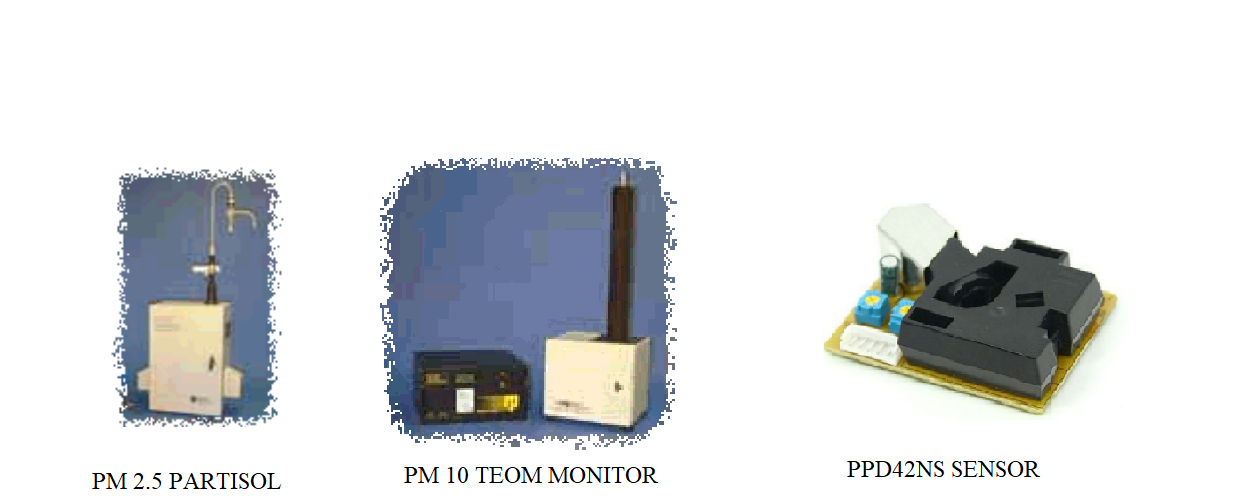
\includegraphics[scale=0.70]{images/figure29.png}
  \end{center}
  \caption{Particulate matter sensor used for measurement}
\label{PM}
\end{figure}

\item DHT11: This is a very low-cost sensor available for temperature and humidity measurement and has a calibrated digital output. The measurement range for temperature is from 0 to 50 degrees Celsius. The device can be integrated with almost all Microcontroller platforms and is considered to be the best choice for many applications.

 \end{enumerate}

 \subsection{Communication Module}
 
 The collected data needs to be transferred to a server and from there to a visualization tool so that user can understand and interpret the data. Selecting the right communication module was hard as the main requirement was to establish a stable connection that will constantly send data over the network. At the initial stage of the research project we used an ESP module for data transfer. The WiFi module, ESP8266, is a highly integrated SOC that meets the requirement of efficient power usage, compact design and reliable performance\cite{Systems2018}. The ESP module can be connected to a processor or it can also operated independently as the module itself acts as a microcontroller unit. Unlike the sensor modules connected to an Arduino module which needs a 5V power supply for its operation, this module needs a 3.3V power supply. The ESP module comes with installed firmware and it communicates using AT commands. On entering AT command in the serial monitor, the output would come as 'OK' if there is a successful connection. 

 %This firmware can be replaced with user's own code which gives the power of flexibility of connecting with any IOT platform. The arduino platform supports the programming of ESP module which makes the integration much easier. The code can be written in the Arduino IDE and can be flashed into the ESP board by connecting it separately. 
 However, this module failed to provide a reliable connection to the network and it also faced issues with power-up when all the sensors were connected. This became a challenge for data transfer so we chose a more efficent and reliable module called \lq{WEMOS D1 mini}\rq. WEMOS is a miniature microcontroller based on an ESP8266 and can be easily integrated with Arduino. The development board has eleven digital input/output pins and one analog pins. The programming for the device is done through the Arduino IDE and flashed via the USB connector. The programming for the system was very similar to the earlier ESP module and it provided a stable connection.
 
 % the having a stable network connection for data transfer.
 
 \iffalse
 The circuit for the ESP flashing is as shown in figure \ref{cir} which is a voltage divider circuit.

 \begin{figure}[h]
  \begin{center}
  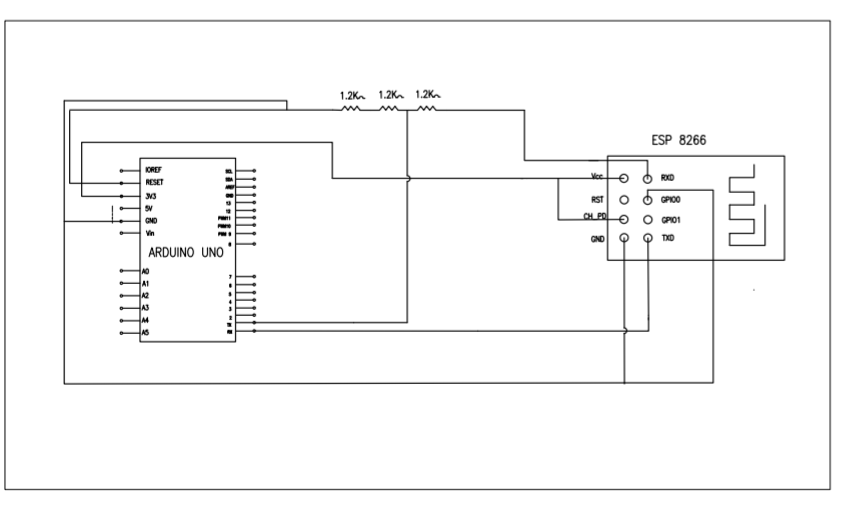
\includegraphics[scale=0.95]{./images/figure11.png}
  \end{center}
  \caption{System Overview}
  \label{cir}
\end{figure}


 When the TX and RX pin of Arduino is connected to TX and RX pin of the WiFi module it becomes in the programming mode and flashing occurs. 
 \fi


 \subsection{System Overview}

 This section will show the integration of the above-mentioned sensors with the Arduino and communication module. After selecting the sensors and processor for the air pollution data measurement the next task was to put together a working system. This was done one step at a time so that troubleshooting will be simpler. The complete circuit diagram of how the components are integrated to the Microcontroller is shown in Figure \ref{circuit}.
 
 \begin{figure}[h!]
  \begin{center}
  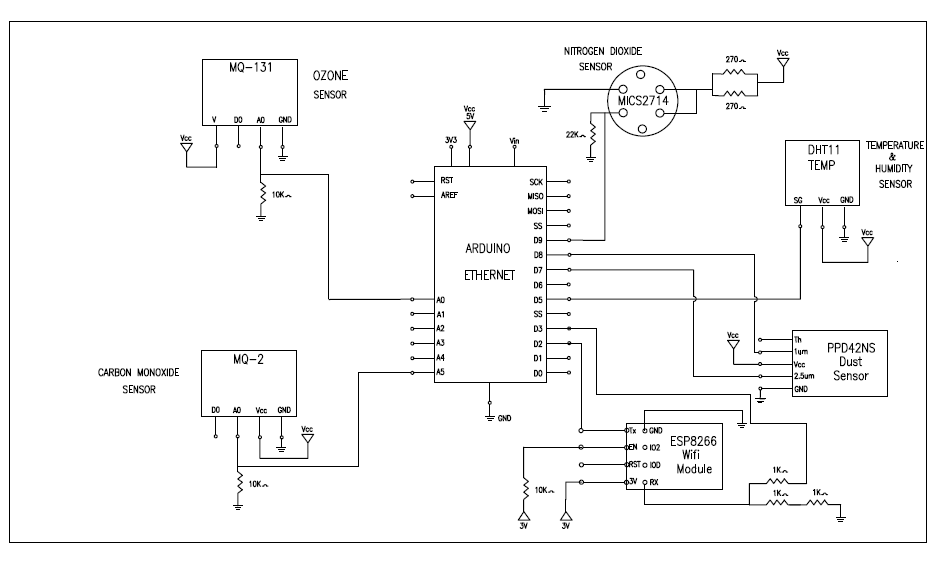
\includegraphics[scale=0.55]{./images/figure5.png}
  \end{center}
  \caption{Circuit diagram of air pollution system}
  \label{circuit}
\end{figure}


\hspace{1 cm}

 Each of the sensors was carefully arranged to reduce spatial interference. The majority of the sensors use heating devices and heat discharges affects the operation of the sensors placed nearby. The initial circuit implementation was done using a wired breadboard. Building the circuit with a breadboard gave the flexibility to work with different arrangements.
\begin{comment}
 \begin{figure}[h]
  \begin{center}
  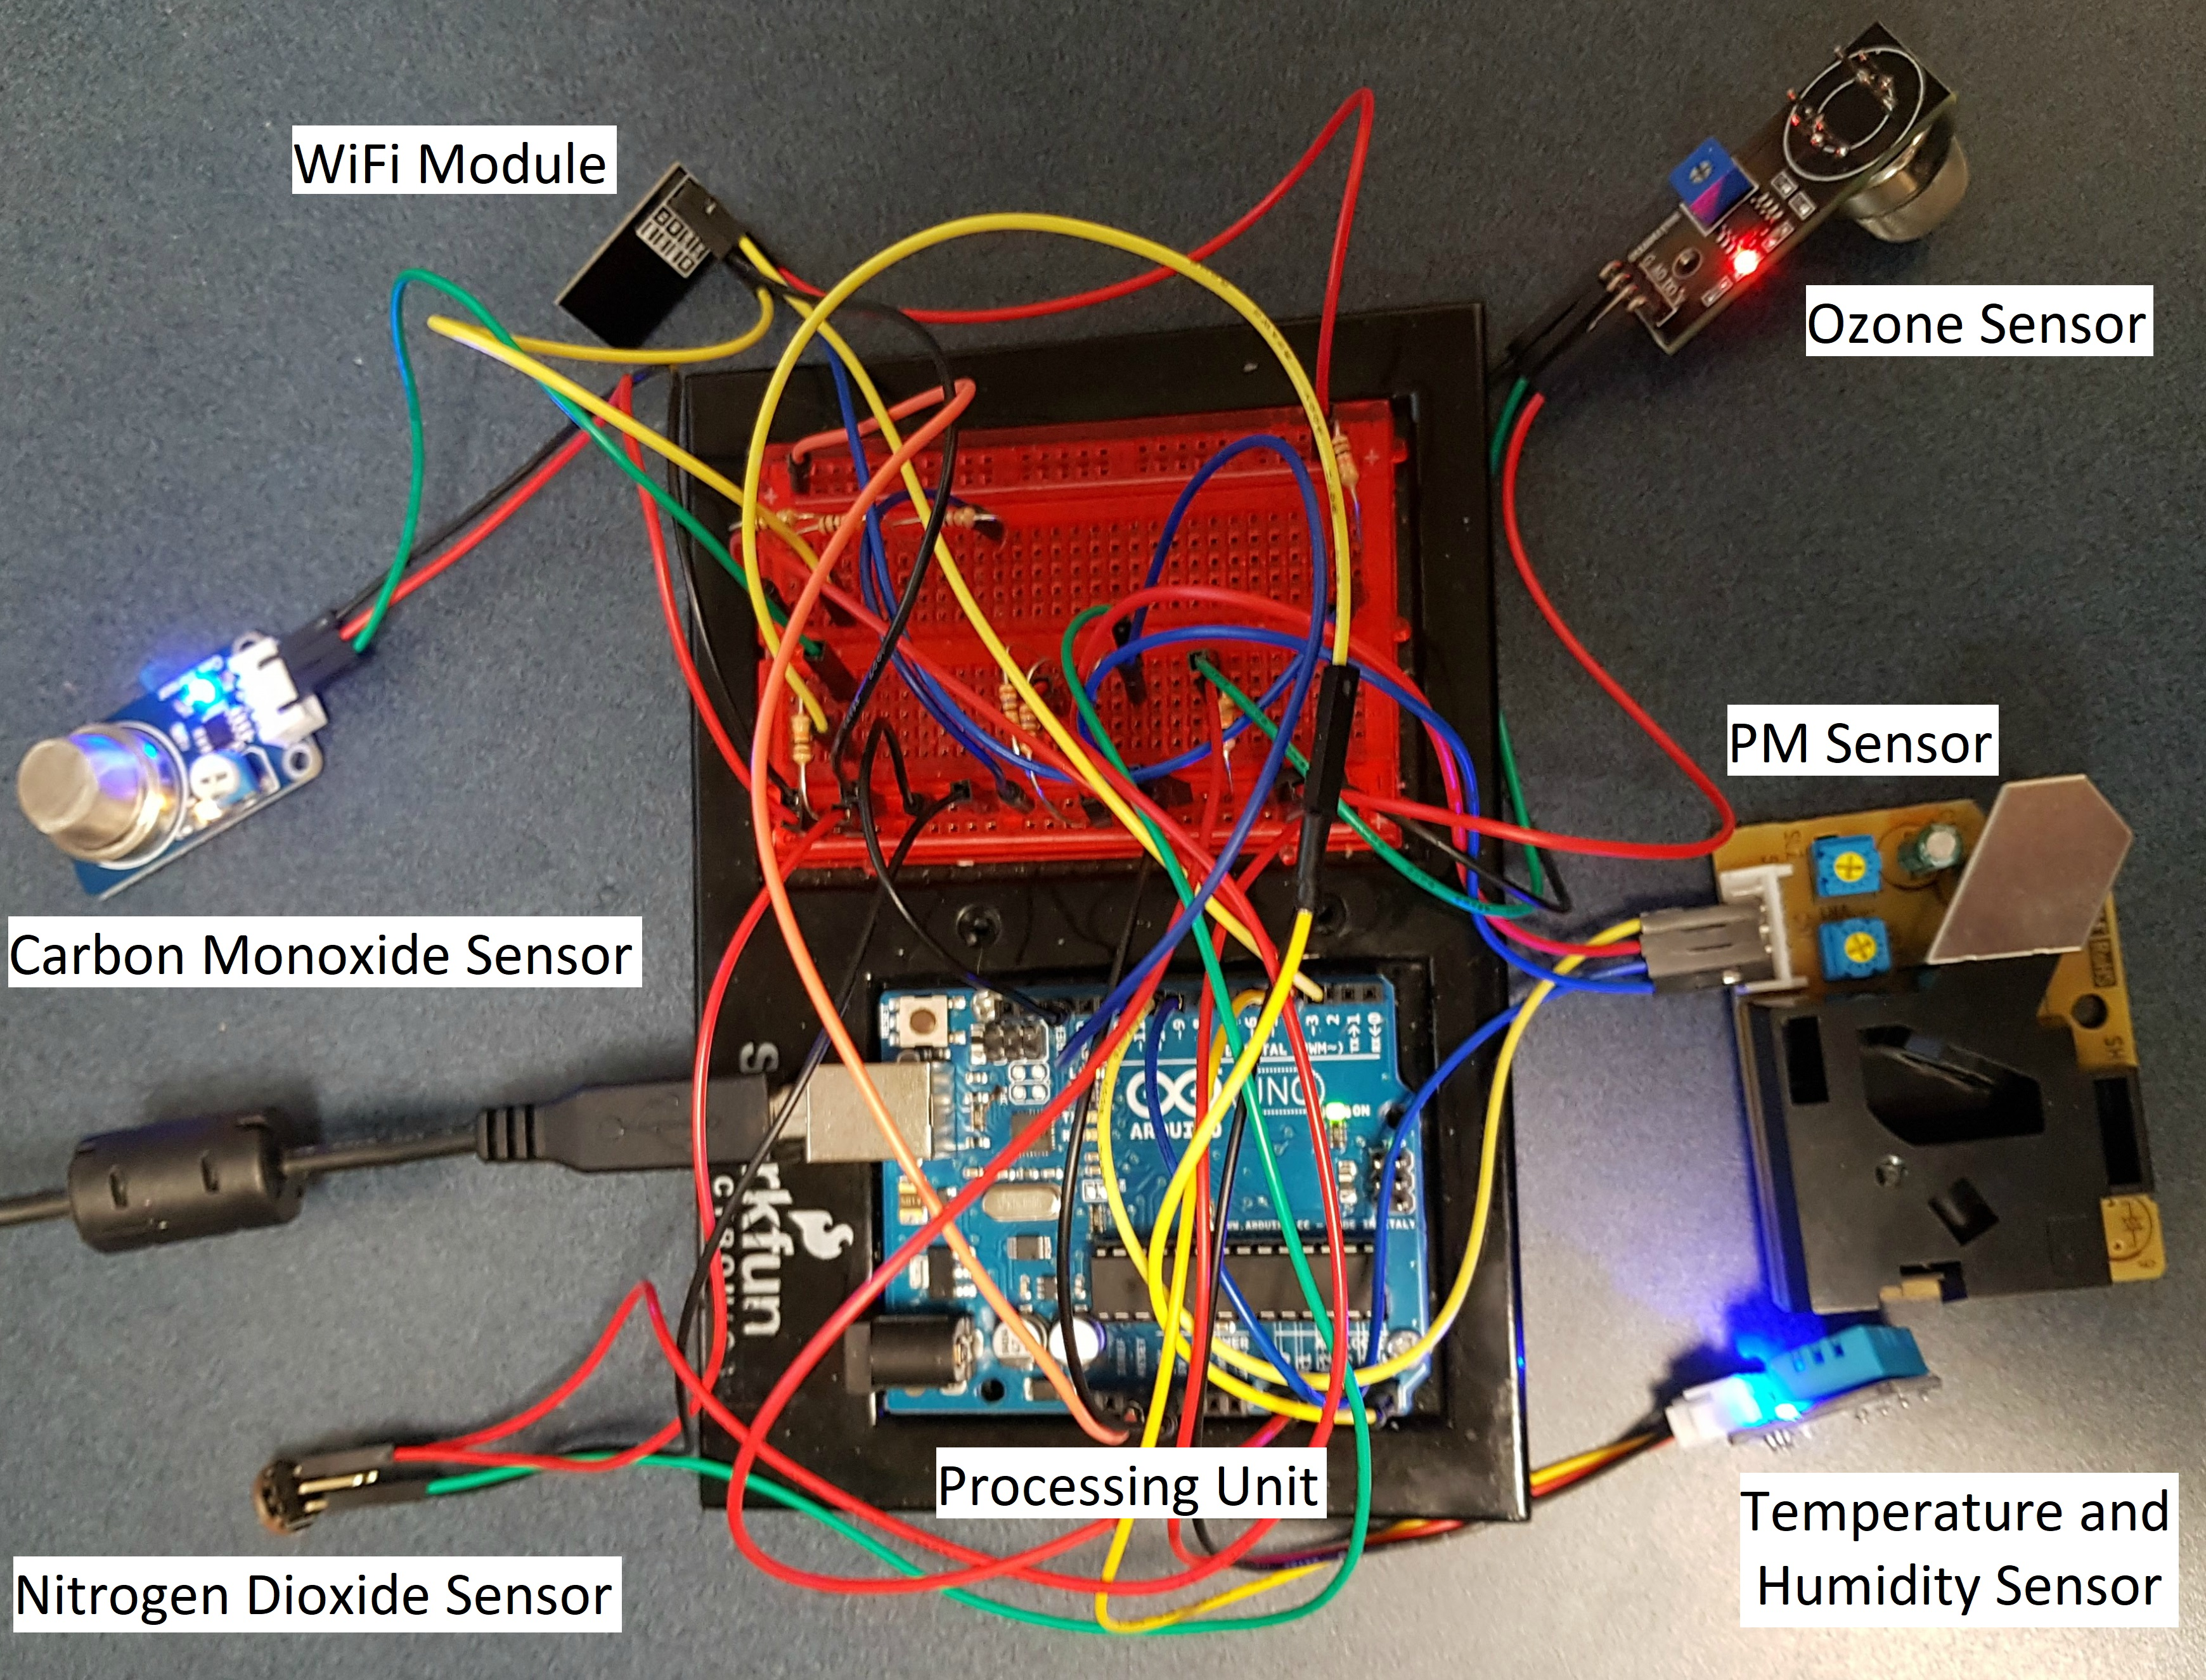
\includegraphics[scale=0.09]{./images/figure14.jpg}
  \end{center}
  \caption{Prototype Implementation}
  \label{prototype}
\end{figure}
\end{comment}
After building the circuit in a breadboard, it was migrated to a Printed Circuit Board (PCB) developed in Flemings Solution Ltd, India. The PCB was designed in such a way that each of the sensors can be plugged into the Arduino board which gave flexibility in case of any damage. 
\begin{comment}
  

\begin{figure}[h]
  \begin{center}
  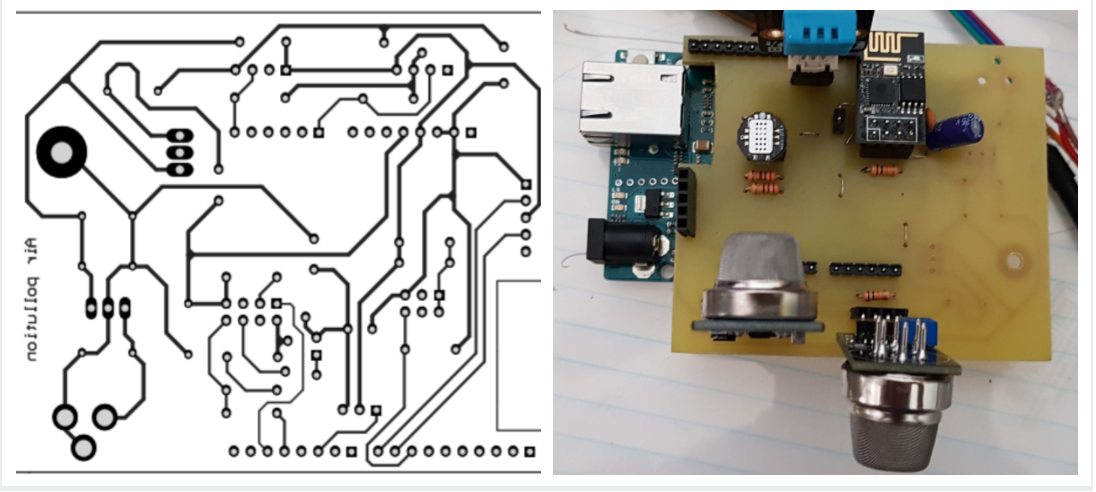
\includegraphics[scale=0.65]{./images/figure18.png}
  \end{center}
  \caption{Printed Circuit Board}
  \label{pcb}
\end{figure}
\end{comment}
 This was done in case of any malfunctioning of sensors or processor, so could be replaced easily. The main advantage of using a PCB design is that all the components are fixed and there is no wiring at all. This produces a stable circuit for the sensor platform.

\section{Software Architecture : Customizable Layered Visualization (CLV)}

The hardware is responsible for the data collection but making the data available to users is done by effective visualization software. The main objective for developing the system was that the data collected should be accessible from anywhere. We developed a customizable layered visualization for the data that potentially involve different stakeholders. We believe that an effective visualization of relevant data is critically important for effectively combating major issues. The software design is driven by the following four key elements:

\begin{itemize}

\item Stakeholder specific  visualization.

\item Author-guided and user-driven interactivity.

\item Hierarchical approach to visualization.

\item Providing options for users.

\end{itemize}



\subsection{Framework}

The pollution monitoring stations collect huge amounts of data for pollutants and there are various ways to make people aware about this data. There can be different groups of users who will have access to the data which can be categorized as layman, data scientists (educators or researchers) who will be analyzing on the data, and the policy or lawmakers who will take necessary actions. Accurately identifying the stakeholders with an interest or stake in air pollution data is challenging. The paper on health, safety, and environment  \cite{English2000} categorizes stakeholders in environmental risk decisions into four categories of stakeholders as risk losers, risk gainers, risk perpetrators, and risk managers. 


%Risk losers \cite{English2000} are those who may be adversely affected by environmental risk decision, in terms of health or economic values and risk gainers are those who may be favorably affected by an environmental risk decision, typically through economic gains. The people who create the risk are the perpetrators and those who takes the action against the risk are the risk managers. In a similar way, here we have put forward an approach of visualization based on the different stakeholders, in which we have classified into three categories: risk losers, risk analyzers and risk managers. 

\lq{Risk losers}\rq are those who are susceptable to pollution which includes the general public or the society as a whole and \lq{risk gainers}\rq are those who gain  favorable outcomes from environmental risk  decision mainly through economic gain. \lq{Risk prepetrators}\rq are those who create risk and \lq{risk managers}\rq are those who implement laws and regulations by looking at the trends of pollution for a certain period. 
In a similar way, we have also categorized our stakeholders into three main categories as layman, data scientist, and policymakers. We believe this categorization for representing air pollutant data is very efficient as it helps in representing what each stakeholder wants to view in the data.

The visualization should be simple for users and be able to drive the user to details of interest. It should not necessarily represent all the data in a single screen, which could be confusing to users and will lose the interest of different stakeholders. The user should be able to choose what data they need to view. If this approach is included in visualization design, the data that different stakeholders are looking for will be passed to them in an efficient manner. %We have summed up this visualization idea in the paper that we tried in 2018 \cite{Saju2018(1)}.

\subsection{Implementation of CLV of Air Pollution Data}

The complete software implementation for the visualization software was created using a combination of Node.js and Python. The framework for the software is shown in Figure \ref{frameworksoft}. In Figure \ref{frameworksoft} the back-end and the front-end of the software is clearly shown and how it is connected with each other. The front-end is the representation layer with which the user interacts to get an output, for example, the webpage which represents information demanded by the user. The back-end of software can be described as what makes the front end work and it deals with the server-side. The back-end mainly  focuses on database, scripting, and architecture.
\begin{figure}[h]
  \begin{center}
  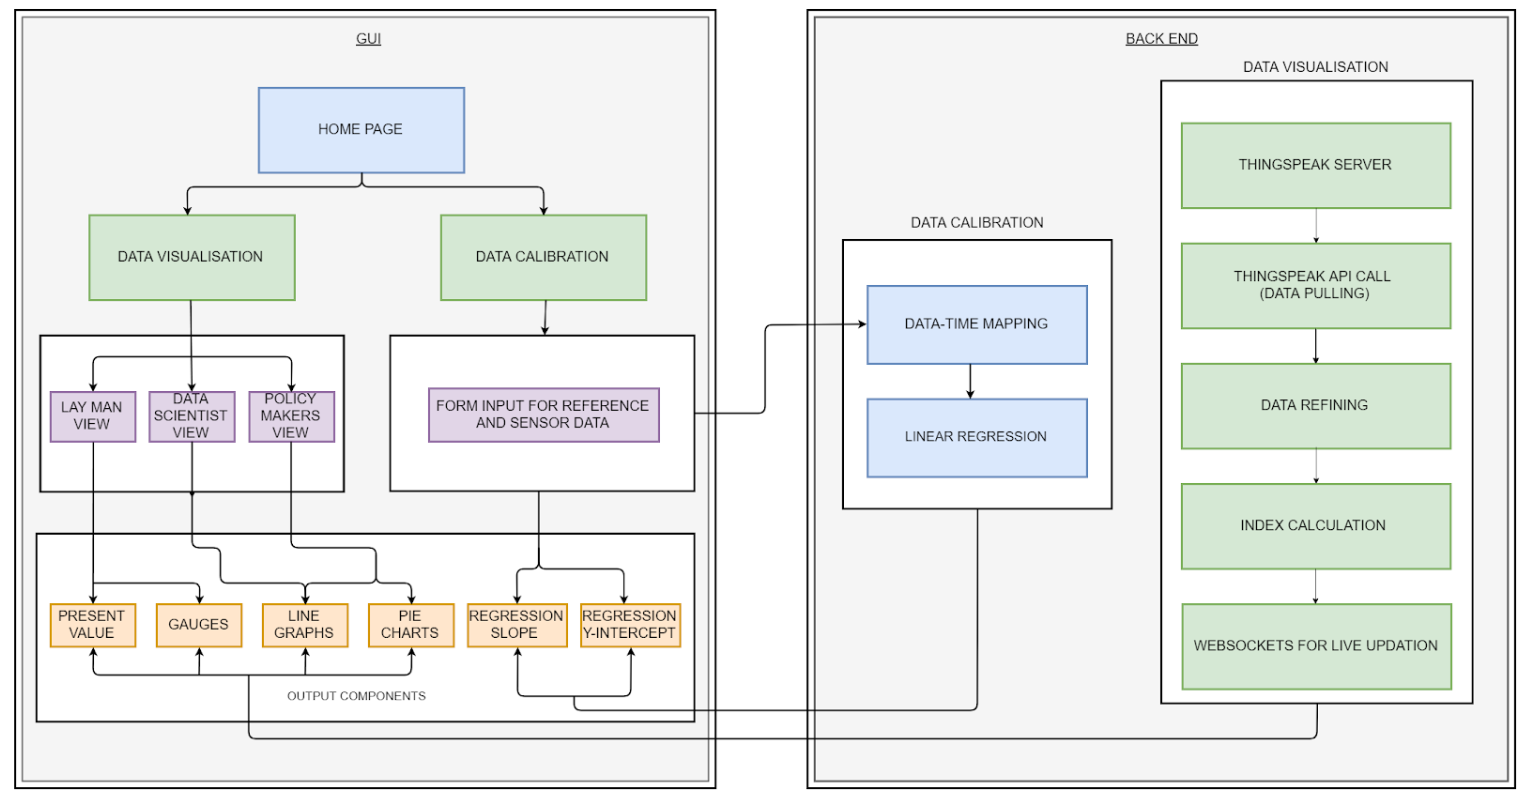
\includegraphics[scale=0.58]{./images/figure33.png}
  \end{center}
  \caption{Software Architecture}
  \label{frameworksoft}
\end{figure}

\hspace{1 cm}


According to the classification of stakeholders, each user group is looking for different views of the data. For example, the data could be represented in the form of huge spreadsheets or documents. There are different methods for visualization for large data sets, such as heat-maps, bubble plots, box plots, bar graphs or a plane graphs. The most common method for displaying complex data is a graphical method, which can show the data corresponding to a certain time or day. We believe that instead of visualizing the entire data set through graphs or plots, it would be easier for the layman to interpret the data if it is a single instantaneous value. The  representation implemented for the lay man stakeholder is as in Figure \ref{view1}, which shows a single value for the pollutant. The implemented representation of the data is easy to understand and it shows the concentration that each pollutant adds to atmosphere. The idea of this kind of visualization is that the user who falls into layman category simply needs to read the data from the display.

\begin{figure}[h]
  \begin{center}
  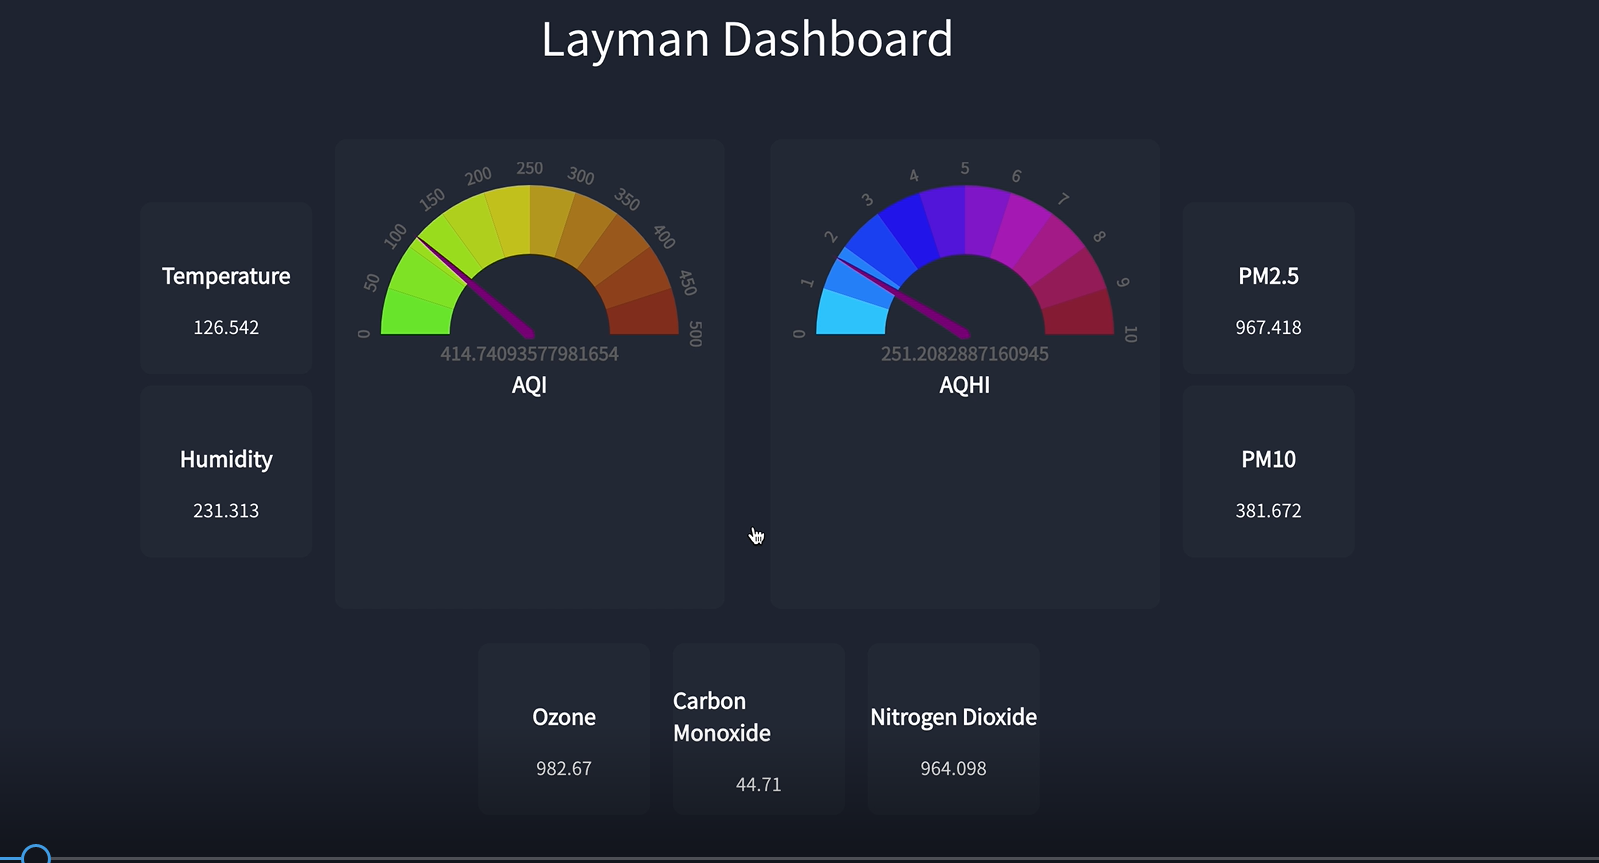
\includegraphics[scale=0.45]{./images/figure14.png}
  \end{center}
  \caption{Dashboard for Layman category}
  \label{view1}
\end{figure}

\hspace{1 cm}

The next data visualization implementation is done for the  data scientist or researcher and is as shown in Figure \ref{view2}. The ideal way to represent this more detailed view of information is through line graphs to show the values obtained over a range of time. The measured value of pollutants could be seen when the pointer hovers over the graph. These graphs are updated every time the source data is updated by the system, as researchers need to know real-time data to understand the scenario. 


\begin{figure}[h]
  \begin{center}
  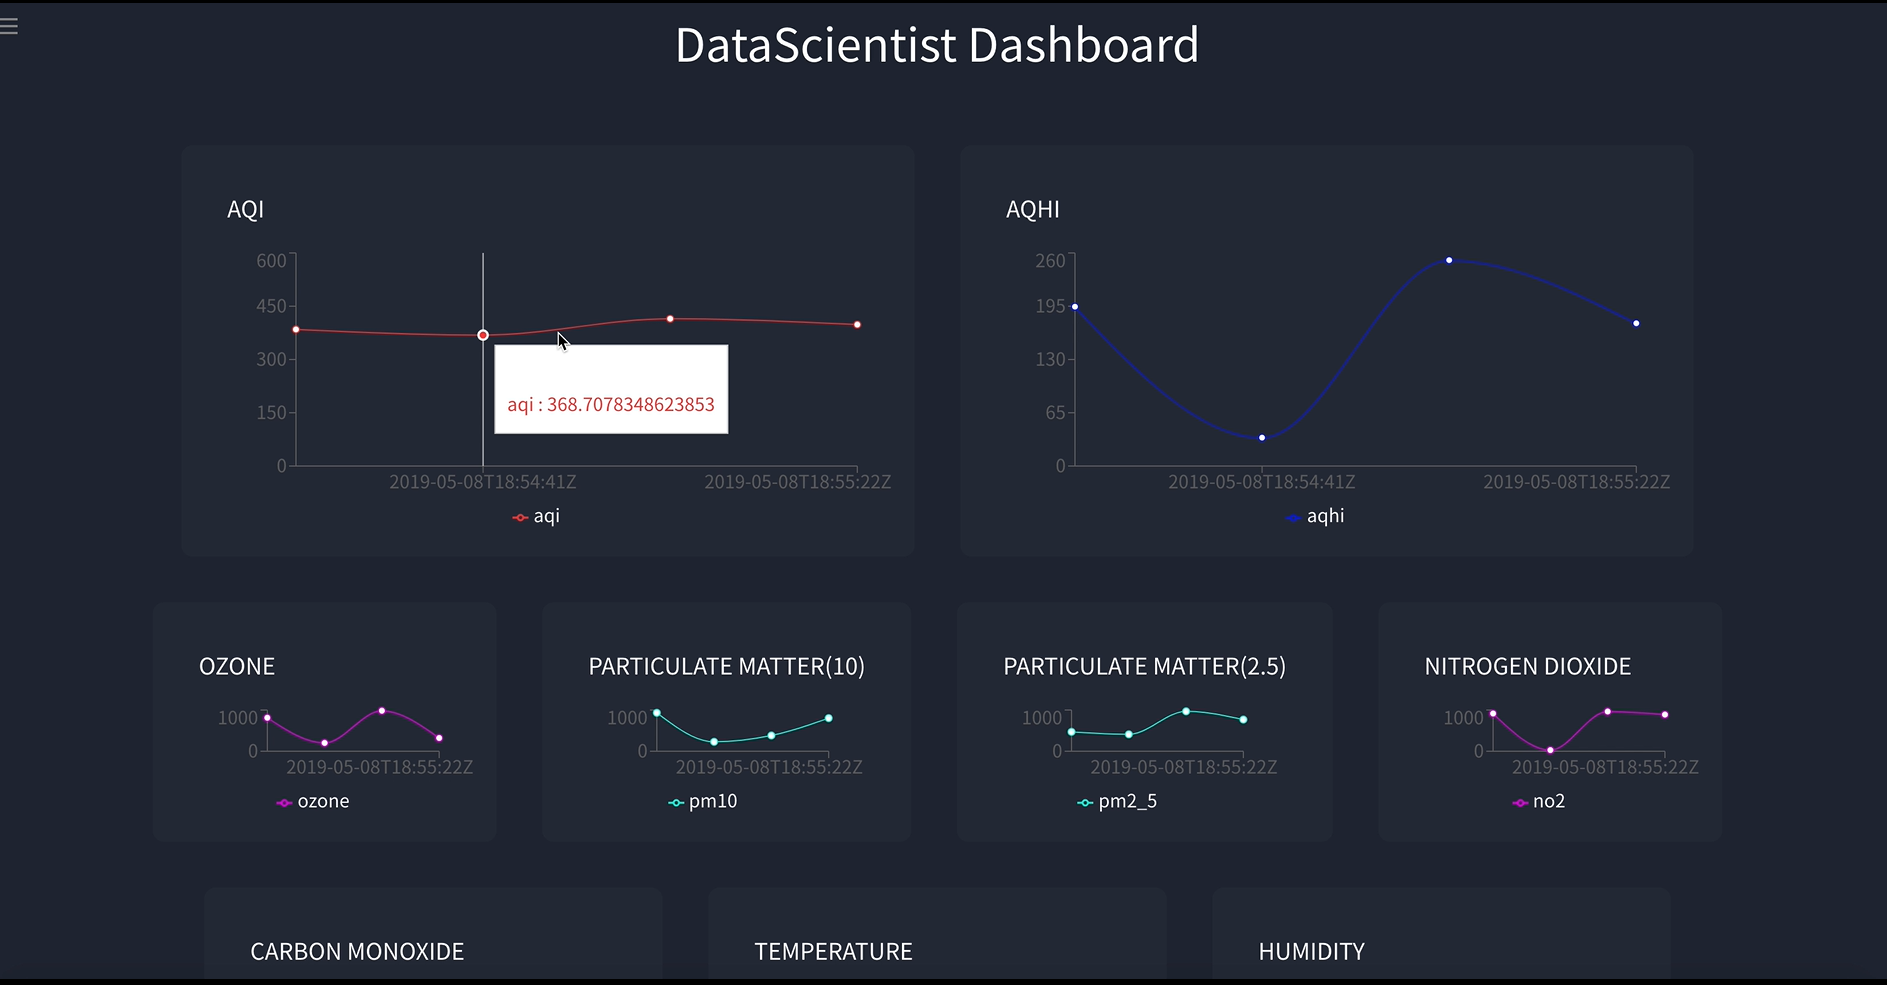
\includegraphics[scale=0.40]{./images/figure15.png}
  \end{center}
  \caption{Dashboard for Data Scientist or researcher}
  \label{view2}
\end{figure}


\hspace{1 cm}

The last categorization of users are the policymakers who implement actions based on changes in the concentration of pollutants. They are responsible for creating or enforcing policies and laws by looking at the pollutant data and hence they are the ones who need to see a combined view of all the pollutants and the trends in data as shown in Figure \ref{view3}.

\begin{figure}[h!]
  \begin{center}
  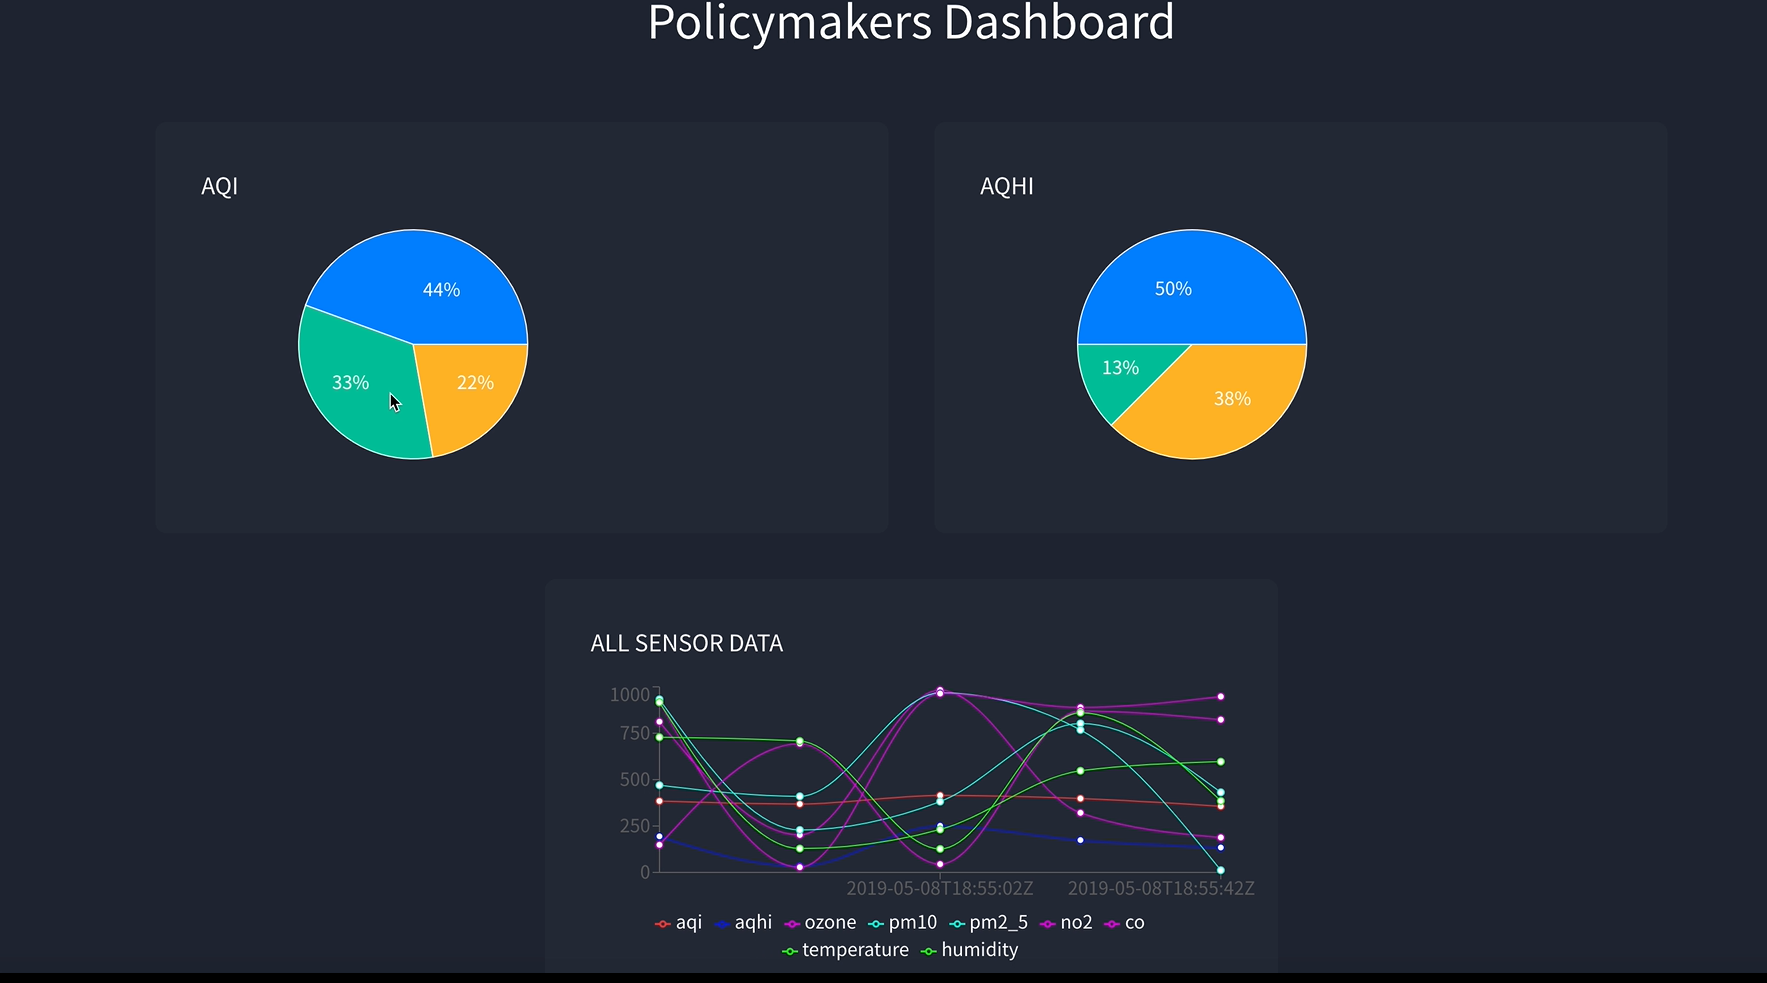
\includegraphics[scale=0.45]{./images/figure16.png}
  \end{center}
  \caption{Dashboard for policymakers}
  \label{view3}
\end{figure}

\hspace{1 cm}

This can be visualized by pie-charts which shows the percentage of each pollutant that contributes to the indexes. There is also a combined line graph that shows concentrations of different pollutants. By looking at the pie-charts and the combined graphs these users would be able to understand the trends and also could identify the pollutants that contribute more to the indexes. 

The idea of such a hierarchial level of visualization is that it changes according to the users or groups who are focusing on these data. Albert Cairo, a renowned information designer claims that the fundamental goal of data visualization should be to make people better informed \cite{Hepworth} \cite{Cairo2014},  similarly we also believe that well communicated data is important for visualization.


\subsection{Data Storage - ThingSpeak}

The previous section demonstrated how the data can be visualized. One other aspect to be noted is where does the data get stored? The pollutant data that we collect from each system needs to be stored so it can be retrieved when needed. To implement this we use an open source IoT platform called ThingSpeak \cite{thingspeak}. This is a visualization service that allows the system to aggregate, analyze, visualize, and store the sensor data \cite{thingspeak}. ThingSpeak can allow many users to integrate their systems with other systems for collective and cooperative analysis of sensor data and promote citizen science in solving important local, regional or global problems. It offers a \lq{hub}\rq model for data repository and a set of APIs for accessing and using the sensor data for analysis and interpretation. We have used the data repository service of ThingSpeak (which is a free) to act as our server. The data transferred from WEMOS is stored using an API key provided by ThingSpeak and updated when new data is available. The data can be downloaded in the form of csv file which is simple to use in the subsequent analysis.
%to display the results. As soon as the value is transferred to Thingspeak, it can immediately draw graph showing online visualization. We have used eight channels of Thingspeak for the graph representation of all the pollutants measured by the sensors and the AQI and AQHI metrics.

\section{Summary}

The implementation of a sensor system using hardware and software along with their integration have been explored. We have discussed the sensors selected and how these connect to the Arduino platform. The different stakeholders are identified and how the data is represented for each classification has been discussed. The next concern is the quality of data collected, which will be explained in the next chapter.

